\documentclass[11pt,a4paper,oneside]{article}
\usepackage[a4paper,top=2cm,bottom=2.5cm,left=2.5cm,right=2cm]{geometry}
\usepackage[T1]{fontenc}
\usepackage[utf8]{inputenc}
\usepackage[italian]{babel}
\usepackage{frontespizio}
\usepackage{graphicx}
\usepackage{subfig}
\usepackage[italian]{varioref}
\usepackage{url}

\begin{document}
\baselineskip 22pt

%Indice%
\tableofcontents\thispagestyle{empty}\clearpage

\section{Introduzione}
\pagenumbering{arabic}
\baselineskip 12pt
Negli ultimi anni c'è stato un discreto aumento dell'occupazione femminile in Italia che, da poco più del 33\% nell'anno '77, è arrivata nel 2019 a superare il 50\%. Per quanto il miglioramento sia da apprezzare, la metà della popolazione femminile è ancora da considerarsi disoccupata, e anche se la maggior parte in questa percentuale è probabile che siano le donne più giovani, ancora dietro agli studi, è necessario che il tasso continui ad aumentare. A livello europeo, infatti, il nostro paese si trova tra gli ultimi posti per quanto riguarda il tasso di occupazione femminile, mantenendo un forte divario tra uomini e donne, e di conseguenza privandosi di un'importante componente lavorativa.

In questo studio, cerchiamo di analizzare l'andamento del tasso preso in considerazione, per arrivare a una previsione di come muterà nel futuro prossimo.

\section{Tabella dei dati}
La tabella è stata recuperata dal sito \url{http://dati.istat.it/Index.aspx?DataSetCode=DCCV_TAXOCCU1}, selezionando i dati disponibili relativi al sesso femminile, alla fascia di età 15-64 anni, per ogni trimestre da gennaio del 1977 a settembre del 2019. Il dataset è stato esportato in formato csv, e sono stati prese in considerazione soltanto le colonne indicanti il trimestre e il tasso occupazionale relativo. Sono presenti in tutto 171 osservazioni.\\
Dopo aver importato sul software il file csv, effettuiamo la conversione dei dati in serie storica:
\begin{verbatim}
> to.data = read.csv("tabella.csv",row.names=1)
> head(to.data)
> to = ts(to.data,frequency=4,start=c(1977))
\end{verbatim}
Siamo adesso pronti per il nostro studio.
\section{Analisi dei dati}
Iniziamo con la visualizzazione della nostra serie storica nella figura~\ref{fig:tsplot}: possiamo subito notare la presenza di un forte trend ascendente, mentre non è molto evidente una stagionalità.  Di fatto, se osserviamo attentamente, possiamo vedere che le fluttuazioni della serie nel grafico, identificate dai lievi picchi, sono tutte in corrispondenza di un anno solare. Soprattutto nei primi anni disponibili, fino almeno al 2000, i picchi sembrano molto simili tra loro, indicando quindi che una stagionalità, seppur probabilmente di ordine di grandezza piccolo, deve essere presente.
\begin{figure}[h]
\centering
\subfloat[][\emph{Visualizzazione dell'andamento dei dati}\label{fig:tsplot}]
{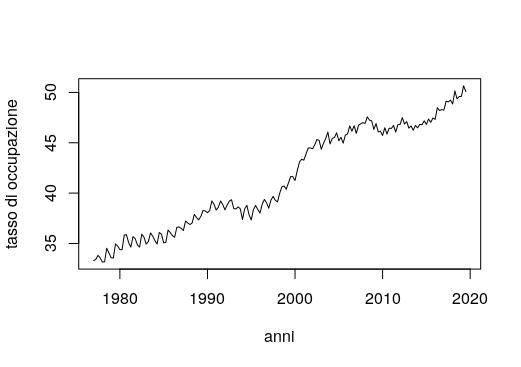
\includegraphics[width=0.5\textwidth]{images/tsplot}}
\subfloat[][\emph{Funzione di autocorrelazione}\label{fig:acf}]
{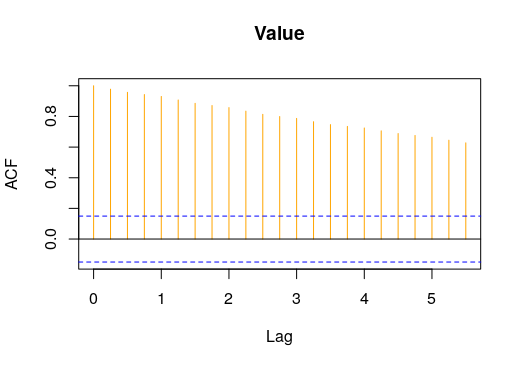
\includegraphics[width=0.5\textwidth]{images/acf}} \\
\caption{}
\label{fig:grafici}
\end{figure}

Andiamo, quindi, ad analizzare la funzione di autocorrelazione e anche da essa vediamo che la componente di periodicità sembra non esserci (fig.~\ref{fig:tsplotDiff}). Sappiamo, però, che questa funzione è di dubbia interpretazione se in presenza di un forte trend, e proviamo quindi a visualizzare la serie al netto del trend: 
\begin{verbatim}
> plot(diff(to))
> acf(diff(to),col="orange")
\end{verbatim}
Si nota già meglio che ogni anno è visualizzato da un picco, sottolineando quindi la presenza di stagionalità. Questi picchi sono ben distinti per i primi anni, almeno fino al 2003, per poi cambiare andamento e suddividersi in picchi più confusi tra i vari trimestri. Dalla funzione di autocorrelazione, poi, sembra che così una componente stagionale possa essere effettivamente presente: in corrispondenza dell'inizio di ogni periodo, vediamo che il valore di acf si staglia al di sopra degli altri valori, evento che era stato mascherato nei grafici precedenti dalla presenza di un trend accentuato.
\begin{figure}[h]
\centering
\subfloat[][\emph{Visualizzazione dei dati al netto del trend}\label{fig:tsplotDiff}]
{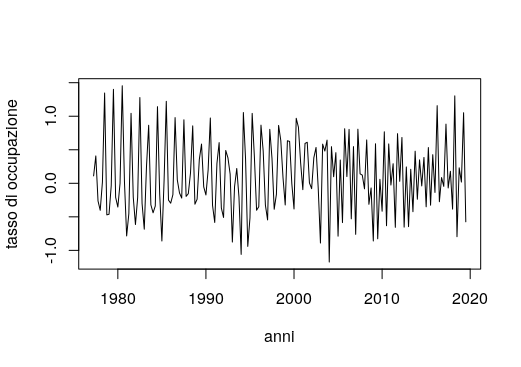
\includegraphics[width=0.5\textwidth]{images/tsplotDiff}}
\subfloat[][\emph{Funzione di autocorrelazione al netto del trend}\label{fig:acfDiff}]
{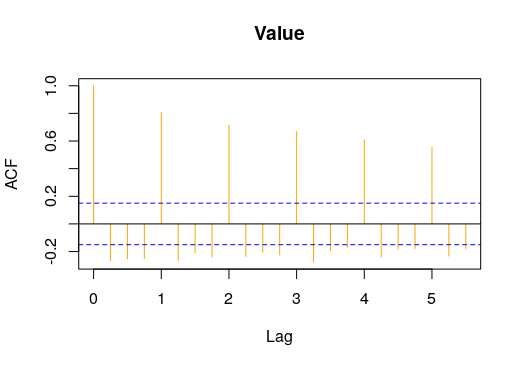
\includegraphics[width=0.5\textwidth]{images/acfDiff}} \\
\caption{}
\label{fig:graficiDiff}
\end{figure}

Proviamo, ora, a visualizzare l'andamento annuale della serie, sovrapponendo i valori a disposizione di ogni anno (fig.~\ref{fig:plotPeriodi}). Sembra ancora che ci sia una lieve periodicità, per cui verso la metà di ogni anno il tasso sembra crescere per poi riabbassarsi leggermente: questo fenomeno, dovuto probabilmente alla richiesta maggiore di lavoro durante la stagione estiva, così come alla fine dell'anno per le feste natalizie, si registra con fluttuazioni a livelli di cifre decimali nel tasso registrato ogni trimestre, e per questo motivo non viene facilmente distinto.
\begin{figure}[h]
\centering
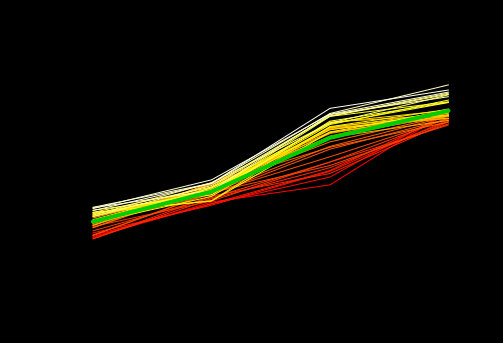
\includegraphics[width=0.4\textwidth]{images/plotPeriodi}
\caption{Andamento annuale della serie}
\label{fig:plotPeriodi}
\end{figure}

\subsection{Decomposizione della serie}
uv

\section{Conclusioni}


\end{document}